\documentclass{beamer}
\usepackage{graphics}
\usepackage{url}
\usepackage{ulem}
\usepackage{beamerthemesplit}
\usepackage{hyperref}
\usepackage{wrapfig}
\usepackage[spanish,activeacute]{babel}
\usepackage[utf8]{inputenc}
\usepackage{listings}
\usepackage{color}
\usetheme{Warsaw}
\usepackage{pstricks}
\lstset{breakatwhitespace=true,
language=C++,
columns=fullflexible,
keepspaces=true,
breaklines=true,
tabsize=3, 
showstringspaces=false,
extendedchars=true}


\title{NVIDIA CUDA}
\subtitle{Introducción y Ejemplos.}
\author{Jonathan Antognini C.}
\institute[]{Universidad Técnica Federico Santa María}
\date{\today}

\begin{document}
    \frame{\titlepage}
    \frame{\tableofcontents}
	\section{Introducción}								%DONE
		\frame{
	\frametitle{Introducción}
	\begin{itemize}
		\item Compute Unified Device Architecture (CUDA), es una tecnología desarrollada por Nvidia Corporation en el 2007.
		\item Soportado de la serie G8X en adelante.
		\item Compilador (nvcc) + conjunto de herramientas de desarrollo en C/C++.
		\item Existen wrappers para otros lenguajes como: Python, Fortran, Java.
		\item El SDK está disponible para Linux, Windows y Mac.
	\end{itemize}
}
						%DONE
	\section{NVIDIA CUDA}								%DONE
		\frame{
	\centerline{Nvidia Cuda}
}
							%DONE
		\subsection{¿Qué es CUDA?}						%DONE
			\frame{
	\frametitle{¿Por qué CUDA?}
	Se intenta explotar las ventajas de las GPU utilizando paralelismo soportado por los múltiples núcleos de una tarjeta gráfica.
	\\
	Las GPU Nvidia son arreglos de multiprocesadores, cada uno de los cuales tiene:
        \begin{itemize}
                \item Varios cores, que ejecutan el mismo programa concurrentemente.
                \item Memoria compartida, y mecanismo de sincronización.
        \end{itemize}
}
						%DONE
		\subsection{Empezando en CUDA}						%DONE	
			\frame{
	\frametitle{Empezando en Cuda}
	Cuda Downloads: Última versión estable: 4.2. Hay un RC 5.0
	\url{http://developer.nvidia.com/cuda/cuda-downloads}
	\begin{itemize}
		\item Instalar toolkit.
		\item Instalar driver compatible.
		\item Instalar SDK.
	\end{itemize}

	Cuda library documentation:
	\url{http://www.clear.rice.edu/comp422/resources/cuda/html/index.html}
}
					%DONE
		\subsection{Arquitectura de CUDA}					%DONE
			\frame{
	\frametitle{Arquitectura de Cuda}
	Para efectos de hardware, la GPU funciona como coprocesador, pudiéndose utilizar de forma simultánea a la CPU y así aprovechar el potencial que puedan
        ofrecer ambas al mismo tiempo. Esta arquitectura de procesamiento paralelo masivo es la que proporciona al GPU su alta capacidad de cálculo.
        \begin{center}
                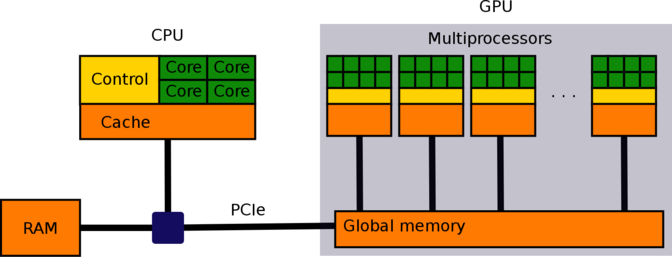
\includegraphics[width=0.6\textwidth]{img/architecture}
        \end{center}
}
					%DONE
			\frame{
	\frametitle{Arquitectura de Cuda}
        \begin{center}
		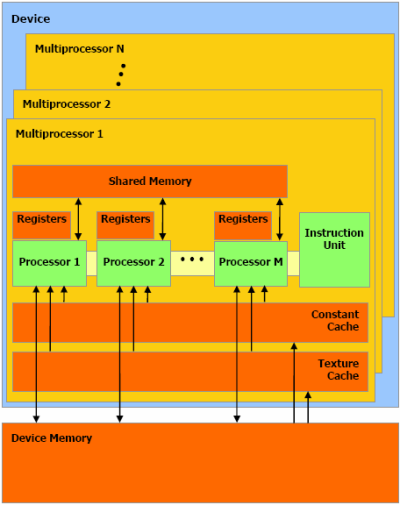
\includegraphics[width=0.6\textheight]{img/HWModel}
        \end{center}
}
					%DONE
			\frame{
	\frametitle{Comunicación entre host y device}
        \begin{center}
		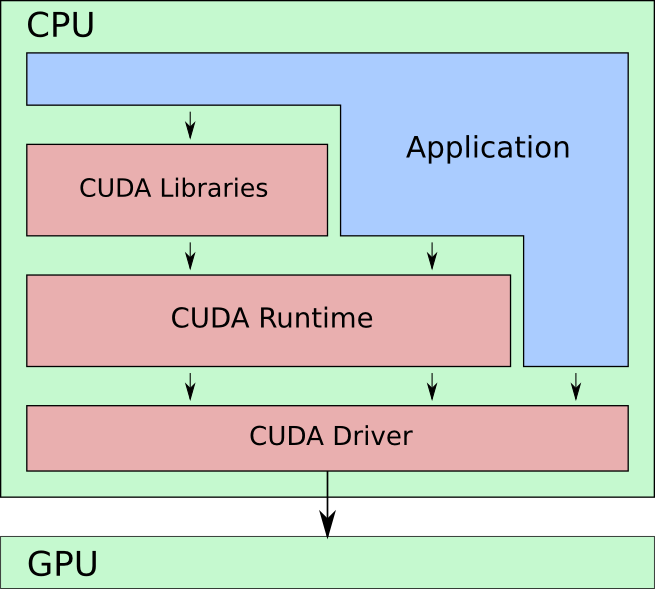
\includegraphics[width=0.6\textheight]{img/application}
        \end{center}
}
					%DONE
		\subsection{Estructura de un programa en CUDA}				%DONE
			\frame{
	\frametitle{Hebras y Bloques}
	\begin{itemize}
		\item Cada hebra se ejecuta en un Streaming processor.
		\item Un bloque es una agrupación fija de hebras.
		\item Cada bloque se ejecuta en un solo Streaming Multiprocessor.
		\item Un SM puede tener asignados varios bloques.
		\item Kernel: función invocada desde la CPU que se ejecuta en la GPU. Recibe como parámetro 
			estructuras que definen la cantidad de bloques y la cantidad de hebras por bloque.
	\end{itemize}
}
						%DONE
			\frame{
	\frametitle{Hebras y Bloques}
}
						%DONE
			\frame{
	\frametitle{Estructura de un programa en CUDA}
	Por lo general, la estructura de un programa en CUDA tiene esta secuencia:
	\begin{itemize}
		\item Generar datos en la CPU.
		\item Copiar datos de la CPU a la GPU.
		\item Realizar cálculo en la GPU.
		\item Copiar los resultados de la GPU a la CPU.
	\end{itemize}
}
					%DONE
		\subsection{Algunos ejemplos}						%DONE
			\begin{frame}[fragile]
	\frametitle{Ejemplos}
	\begin{itemize}
		\item Suma de vectores.
		\item Histograma.
	\end{itemize}
	%\begin{lstlisting}
	%	__global__ void add(int *a, int *b, int *c) {
	%	        int i = blockIdx.x * blockDim.x + threadIdx.x;
        %		if(i<N)
        %       		c[i] = a[i] + b[i];
	%	}
	%\end{lstlisting}
\end{frame}
						%DONE
	\section{Conclusiones}								%DONE
		\frame{
	\frametitle{Conclusiones}
	\begin{itemize}
		\item CUDA permite sacar provecho a las potencialidades de las GPU's actuales.
		\item Abordar problemas paralelos es más sencillo.
		\item Sin embargo es fácil programar en CUDA, pero es difícil conseguir rendimientos elevados.
	\end{itemize}
}
						%DONE
	\frame{
	\centerline{EOF}
}

\end{document}
